%================================================================================
%=============================== DOCUMENT SETUP =================================
%================================================================================

%\documentclass[lang=ngerman,inputenc=ansinew,fontsize=10pt]{ldvarticle}
\documentclass[lang=ngerman,inputenc=utf8,fontsize=10pt]{ldvarticle}
%PACKAGES

\usepackage{parskip}
\usepackage{subfigure}
\usepackage{ifthen}
\usepackage{comment}
\usepackage{color}	
\usepackage{colortbl}
\usepackage{soul}
\usepackage{tikz}
\usetikzlibrary{shapes,arrows}
\usepackage{tabularx}
\usepackage{todonotes}


\definecolor{lightgray}{rgb}{0.75,0.75,0.75}


%================================================================================
%================================= TITLE PAGE ===================================
%================================================================================

\title{Propellerman}
\subtitle{Projektpraktikum Informationsverarbeitung - Projektplan}
\author{Daniel Michalovics, Robin Kusterer, Tobias Maile}

\date{\today}

\begin{document}

\maketitle	
\thispagestyle{empty}
\vspace*{2cm}

\hrule

\section*{Motivation}

Neben vielen Vorlesungen, die sich mit der Theorie befassen, bietet das Praktikum Informationsverarbeitung endlich eine Möglichkeit das bisher erlangte Wissen in die Praxis umzusetzen. Die Aufgabe, ein autonom fliegendes Luftschiff selbstständig zu entwickeln, spornt uns an, da wir unsere eigenen Ideen umsetzen und präsentieren können. Darüber hinaus gewinnen wir durch das Projekt einiges an praktischer Erfahrung hinzu. Der Wettbewerb mit dem anderen Team motiviert uns ebenfalls, da wir natürlich versuchen werden unser Luftschiff mindestens genauso gut zu bauen.




\vspace*{1cm}
\hrule


\begin{figure}[!b]
\centering

\includegraphics[width=0.4\textwidth]{logo_kl.png}
\end{figure}

\newpage

%================================================================================
%================================= CONTENT ===================================
%================================================================================

\section{Beschreibung des Projekts}

\subsection*{Zielsetzung}
Das Ziel des Projekts ist es innerhalb von ca. 3 Monaten einen kleinen autonom fliegenden Zeppelin zu bauen. Dieser soll, ohne menschlichen Eingriff während des Flugs, einen willkürlich zusammengestellten Hindernisparcour durchfliegen und ein kleines Gewicht (Rettungspaket) an eine markierte Stelle transportieren. Der Start- und Endbereich, in dem der Flug startet bzw. endet sind vorgeschrieben. Die Positionen der Hindernisse sind vor Flugbeginn bekannt. Weitere Bedingungen sind, dass das Luftschiff während des gesamten Flugs nicht höher als 2 Meter fliegen darf und dass das Durchfliegen des Parcours nicht länger als 15 Minuten dauern darf.

\subsection*{Ansatz}
\subsubsection*{Aufbau des Luftschiffs}
Der Zeppelin besteht aus einem, mit Helium gefüllten, Ballon und einer Gondel. Die Gondel ist im Prinzip eine Platte aus Styropor auf der folgende Komponenten montiert sind:
\begin{itemize}
\item \textbf{Arduino:} als Steuerzentrale und für die Regelung
\item \textbf{IMU:} zur Bestimmung der Ausrichtung und Flughöhe des Zeppelins 
\item \textbf{Ultraschallwandler und Infrarot-LEDs:} zur Bestimmung der aktuellen Position des Zeppelins
\item \textbf{nRF24L01 Modul:} zur Funkkommunikation mit der Basisstation am Computer
\item \textbf{Drei Motoren mit Propellern, inklusive Motortreibern:} zur Steuerung des Zeppelins
\item \textbf{Elektromagnet:} als Vorrichtung zum Abwurf des Rettungspakets
\item \textbf{Akku:} für die Stromversorgung
\item \textbf{oben beschriebener Ballon:} für den Auftrieb
\end{itemize}

\subsubsection*{Flugsteuerung} 
Der Zeppelin verfügt über drei Gleichstrommotoren, die jeweils einen Propeller antreiben. Einer der drei Motoren ist für das Vorankommen des Zeppelins zuständig und ist daher in Flugrichtung montiert. Ein anderer Motor ist zum Boden gerichtet und wird für die Höhenregelung verwendet. Schaltet man diesen ab, so sinkt der Zeppelin zu Boden. Der dritte Motor, der orthogonal zu den anderen beiden ausgerichtet ist, bewirkt eine horizontale Drehung des Luftschiffs, wobei die Richtung der Drehung von der aktuellen Drehrichtung des Motors abhängt. Um ein dafür ausreichendes Moment zu erzeugen, befindet sich der Motor in einiger Entfernung zum Schwerpunkt der Gondel. Das Aussehen und die Funktion des dritten Motors ist mit dem Heckrotor eines Hubschraubers vergleichbar. Durch die oben beschriebene Anordnung der Motoren ergeben sich zwei translatorische, sowie ein rotatorischer Freiheitsgrad für die Steuerung.

\subsubsection*{Regelung}
\begin{center}
%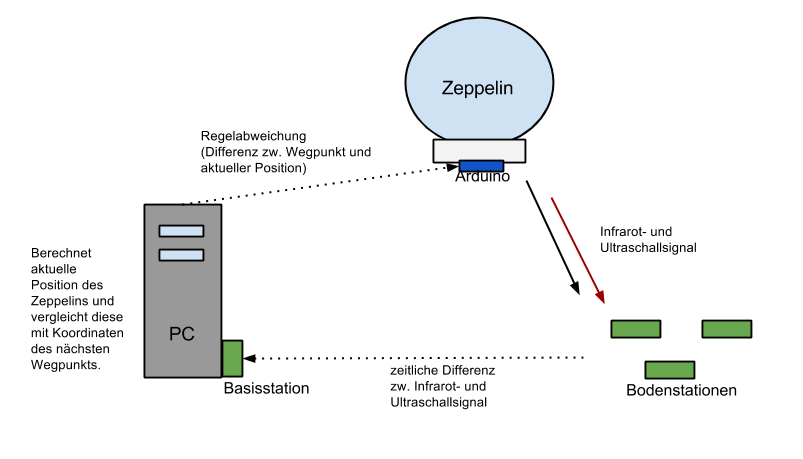
\includegraphics[width=\textwidth]{Regelung.png}
\end{center}
Die Regelung findet hauptsächlich auf dem Arduino-Mikrocontroller der Gondel statt. Als Rückführung dient die Positionsbestimmung über IPS. Dazu sendet die Gondel gleichzeitig ein Infrarot- und ein Ultraschallsignal. Die Bodenstationen empfangen diese Signale zeitlich versetzt und senden die zeitliche Differenz weiter an die Basisstation, die mit einem Computer verbunden ist. Der Computer berechnet zunächst die aktuelle Position des Zeppelins. Anschließend wird die Differenz zwischen der aktuellen Position des Zeppelins und den Koordinaten des nächsten Wegpunkts berechnet,die dann dem Arduino als Regelabweichung übergeben wird.

\subsubsection*{Wegberechnung}
Die Wegberechnung findet am Computer statt. Dafür wird ein Programm erstellt, dass durch Benutzereingaben Informationen zu Start- und Zielbereich, zu Hindernissen auf der Strecke und zur Lage der Abwurfzone für das Rettungspaket erhält. Ein Wegfindungsalgorithmus berechnet daraus eine Folge von Wegpunkten, die das Luftschiff Schritt für Schritt anfliegen soll. Das Programm berücksichtigt ebenfalls die Maße des Zeppelins, um jegliche Kollision mit Hindernissen zu vermeiden.

\subsection*{Erfolgskriterien}
Damit das Projekt gelingt sollten folgende Kriterien erfüllt sein:
\begin{itemize}
\item \textbf{Die Gondel darf ein Gewicht von 100 Gramm nicht überschreiten.}
\item \textbf{Der berechnete Flugweg muss durch gegebene Ziele führen und Hindernissen, unter Berücksichtigung der Größe des Luftschiffs, ausweichen.}
\item \textbf{Das Luftschiff muss in der Lage sein vorgegebene Koordinaten anzufliegen.}
\item \textbf{Die Position des Luftschiffs muss bis auf eine maximal zulässige Abweichung genau berechnet werden können.}
\item \textbf{Die Regelung des Flugs muss stabil und robust gegenüber Störungen, vor allem unerwarteten Luftstömungen, sein.}
\item \textbf{Alle elektronischen Komponenten müssen korrekt miteinander verbunden sein.}
\item \textbf{Alle Komponenten müssen so fest montiert sein, dass sie während des Flugs nicht abfallen.}


\section{Meilensteine}
\end{itemize}


\begin{itemize}
\item \textbf{1. Projektplan bereit für Präsentation}
\begin{itemize}
\item Recherche bereits abgeschlossen
\item Liste aller benötigten Materialien erstellt
\item Lösungsansatz für Projektaufgabe gefunden
\item Projektstruktur vollständig
\item Präsentation erstellt
\end{itemize}
\item \textbf{2. Hardware vollständig und verfügbar}
\begin{itemize}
\item Sammelbestellung bereits geliefert
\end{itemize}
\item \textbf{3. Aktoren und Sensorentest}
\begin{itemize}
\item Aktoren steuerbar
\item Sensoren funktionieren (Testprogramme)
\item IPS testen
\end{itemize}
\item \textbf{4. Navigationssystem eingerichtet}
\begin{itemize}
\item Ultraschall und Infrarot senden und empfangen möglich
\end{itemize}
\item \textbf{5. Gondel fertig gebaut}
\begin{itemize}
\item Befestigung der Hardware
\item Gewichtsverteilung ideal gestalten
\item Verbindung vom Ballon zur Gondel
\item ansteuern der Gondel vom Boden aus
\item Verbindung IPS mit Gondel eingerichtet
\item Motoren sind montiert
\end{itemize}
\item \textbf{6. Erster manueller Flug}
\begin{itemize}
\item Luftschiff lässt ferngesteuerten Flug zu
\item Kommunikation zwischen Komponenten funktioniert
\end{itemize}
\item \textbf{7. Softwareimplementierungen abgeschlossen:}
\begin{itemize}
\item Vorbereitungen auf autonomen Flug 
\item Entwurf der Regelalgorithmen und Pfadfindung
\end{itemize}
\item \textbf{8. Simulation}
\begin{itemize}
\item Errechnen der Positionsfehler für Regelung
\item Anpassungen vornehmen
\end{itemize}
\item \textbf{9. Autonomer Flug}
\begin{itemize}
\item Ballon kommt durchs Ziel
\item Zielpunkte können angeflogen werden
\item Paket kann positionsgenau abgeworfen werden
\end{itemize}
\item \textbf{10. Dokumentation}
\begin{itemize}
\item Simultanes erfassen des aktuellen Fortschritts
\item abschließende schriftliche Darstellung des Projekts
\end{itemize}


\end{itemize}

\section{Projektstruktur (Arbeitspakete)}


\subsection*{Recherche/Materialbeschaffung}

Detailliertes studieren der Herangehensweisen früherer Gruppen, sowie durchstöbern geeigneter Fachliteratur.

Entwurf eines eigenen Konzeptes zur Bewältigung der Aufgabenstellung.

Fristgerechte Organisation passender Materialen.
 

\subsection*{Zusammenfügen der Hardware}

Anschließen einzelner Bauteile an den Computer, Wissenserwerb zum Umgang mit Software.\\
Alle Teammitglieder verschaffen sich einen Überblick über die Funktionsweise der gesamten mechanischen und elektronischen Ausrüstung, sodass jeder in der Lage ist eigenständig Änderungen durchzuführen.

Danach erfolgt zunächst das Zusammenbauen der Gondel. Das Gondelgerüst besteht aus Styropor. Die Positionierung der Motoren muss getestet werden, um eine gleichmäßige Gewichtsverteilung zu erreichen. Grundsätzlich verwenden wir 1 Motor für den Vorwärtsschub, einen Motor für den Auftrieb, sowie einen Motor, der an einer Abstandsstange befestigt wird und für die notwendige Drehung um die z-Achse sorgt.

Erweiterung der IPS Bodenstationen in Zusammenarbeit mit Flying Circus, zur Verbesserung der Funkübertragung. 

\subsection*{Programmierung}
Entwurf einer Softwarearchitektur.
Da die Regelung sehr zeitaufwändig und komplex ist, werden wir zuerst mit Matlab-Simulink simulieren.

Erstellen der einzelnen Programmteile:
\begin{itemize}
\item \textbf{Streckenberechnung:}
	\begin{itemize}
	\item grafische Oberfläche für Benutzereingaben(Start-/Endbereich, Hindernisse, 		Abwurfzone, Maße des Zeppelins)
	\item Algorithmus zur Berechnung einer Strecke von Start bis Ziel bei der das 			Luftschiff nicht mit Hindernissen kollidieren wird
	\item Abtasten der Strecke zu einer endlichen Folge von Wegpunkten	
	\end{itemize}
\item \textbf{Kommunikation:}
	\begin{itemize}
	\item Funkübertragung zwischen Bodenstationen und Basisstation
	\item Datenaustausch zwischen Basisstation und Gondel
	\end{itemize}
\item \textbf{Regelung:}
	\begin{itemize}
	\item Ermittlung der Ausrichtung des Zeppelins aus den Daten der IMU  
	\item Programm zur Berechnung der Regelabweichung am Computer
	\item Implementierung eines PID-Reglers auf dem Arduino-Mikrocontroller
	\item Anpassen der Regelungsparameter durch Flugtests  
	\end{itemize}
\item \textbf{IPS}
	\begin{itemize}
	\item Anpassung und Beseitigung der Fehler
	\end{itemize}
\item \textbf{Treiber zum Ansteuern der Gondel:}
	\begin{itemize}
	\item Ansteuern der Motoren
	\item Ansteuern der Infrarot-LEDs und der Ultraschallwandler
	\item Auswerten der empfangenen Funknachrichten des nRF24L01-Moduls
	\end{itemize}
\item \textbf{Testen}
	\begin{itemize}
	\item Programm, das nacheinander alle elektrischen Komponenten ansteuert
	\item Matlab Programm, das den Regler simuliert
	\item Programm, das Funkmodule ausliest und die Daten am Rechner darstellt
	\end{itemize}
\end{itemize}

Anschließend optimieren und Zusammenfügen.

\subsection*{Test und Evaluation}
\begin{itemize}
\item \textbf{Gondel:}Testen der elektrischen Verbindungen durch Programm, das elektrische Komponenten nacheinander ansteuert 
\item \textbf{Streckenberechnung:} Überprüfen der berechneten Strecke auf Plausibilität.
\item \textbf{Kommunikation:} Auslesen und Überprüfen von übertragenen Daten.
\item \textbf{Regelung:} Simulieren der Regelung in Matlab sowie protokollierte Flugtests mit Auflistung aller Regelungsparameter. 
\item \textbf{IPS:} Überprüfung der berechneten Position des Zeppelins auf Richtigkeit.   
\end{itemize}
Mit den Testflügen wird nach Fertigstellung der Gondel begonnen. 


\subsection*{Dokumentation}
Während des gesamten Projekts wird der Fortschritt überprüft und festgehalten.
Meilensteine müssen fristgerecht erreicht werden. Wöchentlich wird in einem Meeting der aktuelle Fortschritt besprochen und mit dem gewünschten Zeitplan abgeglichen.
Auf Überschreitungen der gesetzen Limits muss umgehend reagiert werden.


Nach dem Wettflug erfolgt die Ausarbeitung des Projekts.


\section{Aktivitäten- / Zeitplan}

\begin{center}
\begin{footnotesize}
\setlength{\arrayrulewidth}{1,05pt}
\begin{tabular}[htb]{|m{0,48\textwidth}|p{.05cm}|p{.05cm}|p{.05cm}|p{.05cm}|p{.05cm}|p{.05cm}|p{.05cm}|p{.05cm}|p{.05cm}|p{.05cm}|p{.05cm}|p{.05cm}|p{.05cm}|p{.05cm}|p{.05cm}|p{.05cm}|p{.05cm}|p{.05cm}|p{.05cm}|p{.05cm}|p{.05cm}|p{.05cm}|}
\hline
\textbf{Monat}& \multicolumn{4}{|c|}{Mai} & \multicolumn{5}{|c|}{Juni} & \multicolumn{4}{|c|}{Juli} \\
\hline
\textbf{Woche}&\tiny\textbf{18}&\tiny\textbf{19}&\tiny\textbf{20}&\tiny\textbf{21}& \tiny \textbf{22} & \tiny \textbf{23} & \tiny \textbf{24} & \tiny \textbf{25} & \tiny \textbf{26} & \tiny \textbf{27} & \tiny \textbf{28} & \tiny \textbf{29} & \tiny \textbf{30}\\
\hline

\rowcolor{lightgray} \textbf{Recherche und Materialbeschaffung}& \cellcolor{red} &\cellcolor{red} & & & & & & & & & & & \\
\hline
\rowcolor{lightgray} \textbf{Zusammenfügen der Hardware}& &\cellcolor{red} &\cellcolor{red} &\cellcolor{red} & & & & & & & & & \\
\hline
\rowcolor{lightgray} \textbf{Programmierung}& & &\cellcolor{red} &\cellcolor{red} &\cellcolor{red} &\cellcolor{red} &\cellcolor{red} &\cellcolor{red} &\cellcolor{red} &\cellcolor{red} & & & \\
\hline

\rowcolor{lightgray} \textbf{Test und Evaluierung}& & & & & &\cellcolor{red} &\cellcolor{red} &\cellcolor{red} & &\cellcolor{red} & & &\\
\hline
\rowcolor{lightgray} \textbf{Päsentation}&\cellcolor{red} & & & &\cellcolor{red} & & & & & & & &\\
\hline
\rowcolor{lightgray} \textbf{Dokumentation}&\cellcolor{red} &\cellcolor{red} &\cellcolor{red} &\cellcolor{red} &\cellcolor{red} &\cellcolor{red} & \cellcolor{red} & \cellcolor{red} & \cellcolor{red} &\cellcolor{red} &\cellcolor{red} &\cellcolor{red} &\cellcolor{red}\\
\hline
\rowcolor{lightgray} \textbf{Meilensteine (werden jeweils zum Ende der KW fällig)}&1 &2 &3 &4 &5 & & &6 &7 &8&9 & & \\
\hline

\end{tabular}
\end{footnotesize}
\end{center}



\section{Aufwandsabschätzung}

Für einen geregelten Arbeitsablauf müssen die Arbeitspakete sinnvoll auf- und eingeteilt werden.
Während auf der einen Seite die einzelnen Komponententests und die Software Programmierung aufteilbar ist, wird es auch zu Knotenpunkten kommen an denen bestimmte Aufgaben abgeschlossen sein müssen. Wichtige Knotenpunkte sind:
\begin{list}{-}{}

\item Zusammenbauen der Gondel.
\item Inbetriebnahme der Gondel.
\item Kommunikation der einzelnen Programme -> Bodenstation - Gondel - IPS.
\item Testen der Regelung am realen Objekt
\end{list}

Diese Punkte werden sehr kritisch behandelt, da sie einige Probleme direkt oder im späteren Verlauf bereiten können.


\section{Material- und Kostenplanung}


Zwei wichtige Kriterien, welche bei jedem Bauteil beachtet werden müssen sind Preis und Gewicht, dabei müssen allerdings auch die speziellen Eigenschafften wie
\begin{list}{-}{}
\item Schub (Motoren/Propeller)
\item Laufzeit (Akku)
\item Stabilität (Gerüst)
\item …
\end{list}
eingehalten werden.

Die von Daedalus zur Verfügung gestellten Rohmaterialien sollten zum Erstellen des Gondelgerüstes ausreichen, und den Gewichtsanforderungen entsprechen. Neben der bereits vorhandenen Elektronik
\begin{list}{-}{}
\item Microkontroller
\item Sensorchip (IMU)
\item Motortreiber
\item Ultraschallwandler
\item infrarot LEDs
\item Kabel, Isolierung, …
\end{list}
werden noch folgende Teile benötigt:

\begin{tabular}{|c|c|c|}
\hline
3x Elektromotoren & max 10 Euro & Conrad \\
\hline
min 1x Motorentreiber & etwa 10 Euro & sparkfun \\
\hline
3x Propeller & 1.50 - 8.00 Euro & Conrad \\
\hline
Akku & 9 - 30 Euro & Conrad \\
\hline
\end{tabular}

für den schlimmsten Fall ergäbe dies etwa eine Summe von 104 Euro.

Die Abwurfvorrichtung wird selbst hergestellt aus vorhandenen Materialien.




\section{Risikoanalyse}

Risiken für das Projekt sind stets Verzögerungen und unerwartete Kosten. Dabei sind zu beachten:

\textbf{Inkompatible oder beschädigte Bauteile}
\begin{list}{->}{}
\item Nachbestellungen können lange dauern und sind teuer.
\item alternative Teile verlangen möglicherweise Kompromisse und müssen neu getestet und verstanden werden.
\end{list}
\underline{Fazit:} Frühe Zusammenstellung aller Komponenten und sorgfältige Tests auf Zusammenwirken mit anderen Bauteilen und den Microkontrollern um Probleme früh zu erkennen.


\textbf{Programmfehler}
\begin{list}{->}{}
\item Debugging ist sehr Zeitaufwendig
\item Fehler treten unerwartet auf und riskieren den Erfolg des Projektes
\end{list}

\underline{Fazit:} Die Softwarearchitektur muss gut Überlegt sein, Arbeitsmittel müssen verstanden sein, enge Zusammenarbeit verhindert Probleme bei der Kommunikation der Programme/Programmteile.


\textbf{Ausfälle/ Terminprobleme}
\begin{list}{->}{}
\item Besprechungen, Testphasen können nicht wahrgenommen werden
\item Kollaboration mit anderem Team/Tutoren kommt schwer zustande
\end{list}
\underline{Fazit:} frühe und verbindliche Terminplanung durch gute kommunikation, mittels Skype, Googlekalender, Github, ..., um den Arbeitsverlauf nicht zu verzögern.


\section{Änderungen des Projektablaufes}
Um Änderungen des Projektablaufs zu dokumentieren wird eine Tabelle in GitHub erstellt, auf die alle Teammitglieder lesenden und schreibenden Zugriff haben. Die Tabelle besitzt drei Spalten, die folgende Informationen über die Änderung enthalten: Datum, Maßnahme, Änderungsgrund.

\end{document}
